\documentclass[oneside]{emulateapj}
\usepackage{graphicx}				% Use pdf, png, jpg, or eps§ with pdflatex; use eps in DVI mode
								% TeX will automatically convert eps --> pdf in pdflatex	
\usepackage{xcolor}
\usepackage{hyperref}	
\usepackage[sort&compress]{natbib}
\usepackage[hang,flushmargin]{footmisc}
\usepackage[counterclockwise]{rotating}
\newcommand{\teff}{$T_{\rm eff}$ }
\newcommand{\logg}{$\log g$}
\newcommand{\feh}{$\mathrm{[Fe/H]}$}
\newcommand{\vsini}{$v \sin{i}$ }
\newcommand{\tc}{$T_\mathrm{C}$}
\newcommand{\vmacro}{$v_{\mathrm{macro}}$ }
\newcommand{\gcm}{g cm$^{-3}$}
\newcommand{\kms}{km s$^{-1}$}
\newcommand\todo[1]{\textcolor{red}{#1}}  % gotta have \usepackage{xcolor} in main doc or this won't work


\shortauthors{Bedell et al.}
\shorttitle{Kepler-11}

\begin{document}
\graphicspath{ {figures/} }
\DeclareGraphicsExtensions{.pdf,.eps,.png}

\title{Revision in the mass and radius of Kepler-11's planetary system via precise spectroscopic characterization}

\author{Megan Bedell\altaffilmark{1},
Jacob L. Bean\altaffilmark{1},
Jorge Mel\'{e}ndez\altaffilmark{2},
Sean Mills\altaffilmark{1},
Daniel C. Fabrycky\altaffilmark{1},
Ivan Ram\'{i}rez\altaffilmark{3},
Martin Asplund\altaffilmark{4},
Fan Liu\altaffilmark{4},
David Yong\altaffilmark{4}}

\email{E-mail: mbedell@oddjob.uchicago.edu}

\altaffiltext{1}{Department of Astronomy and Astrophysics, University of Chicago, 5640 S. Ellis Ave, Chicago, IL 60637, USA}
\altaffiltext{2}{Departamento de Astronomia do IAG/USP, Universidade de
S\~{a}o Paulo, Rua do Mat\~{a}o 1226, Cidade Universit\'{a}ria, 05508-900 S\~{a}o Paulo, SP, Brazil}
\altaffiltext{3}{McDonald Observatory and Department of Astronomy, University of Texas at Austin, USA}
\altaffiltext{4}{Research School of Astronomy and Astrophysics, The Australian National University, Cotter Road, Weston, ACT 2611, Australia}


\keywords{stars: abundances, stars: fundamental parameters, techniques: spectroscopic}

\begin{abstract}

The six planets of the Kepler-11 system are the archetypal example of a population of surprisingly low-density transiting planets revealed by the \Kepler mission. We have determined the fundamental parameters and chemical composition of the Kepler-11 host star to unprecedented precision using an extremely high quality spectrum from Keck-HIRES (R$\simeq$67000, S/N$\simeq$260 at 600 nm). Contrary to previously published results, our spectroscopic constraints indicate that Kepler-11 is a young main-sequence solar twin. The revised stellar parameters raise the densities of the Kepler-11 planets by about 30\%, making them more typical of the emerging class of ``puffy'' close-in exoplanets. We obtain photospheric abundances of 22 elements and find that Kepler-11 is enhanced in refractory materials relative to the solar abundance pattern. We additionally analyze the \Kepler transits and transit timing variations (TTVs) using a photodynamical model and discuss the tension between spectroscopic and TTV-based stellar density estimates.

\end{abstract}

\section{Introduction}

Five years after their initial discovery, the six planets of the Kepler-11 system remain a crown jewel of \Kepler science results \citep{Lissauer2011}. All six planets orbit a Sun-like host star at low eccentricies in a largely co-planar, tightly packed configuration. The formation and long-term stability of the system remains an open question \citep[see e.g.][]{Ikoma2012, Hands2014, Mahajan2014}. Kepler-11 is regarded as the prototypical example of a ``System with Tightly-packed Inner Planets'' (STIP), a class of \Kepler multi-planet systems which offer a surprising counterpoint to our own solar system's architecture. Given the low geometric probability of finding a six-planet transiting system, Kepler-11 is a valuable and rare opportunity to study in detail a common population of exoplanets.

In addition to their unusually tight system architecture, the Kepler-11 planets are noteworthy in another sense: their measured masses and radii place them among the lowest-density super-Earths known to date. Transit timing variations (TTVs) have been measured for all six planets. In the discovery paper, \citet[][hereafter L11]{Lissauer2011} derived mass constraints for the five inner planets based on TTVs from six quarters of \Kepler data. \citet{Migaszewski2012} reanalyzed the same data using a photodynamical model and found similar results, with an additional constraint on the outermost planet mass. The system was later revisited by \citet[][hereafter L13]{Lissauer2013} using fourteen quarters of \Kepler data. All three analyses estimate mean densities of $\leq$ 0.5 $\rho_{\earth}$ for all planets in the system, implying a considerable gas envelope on even the smaller super-Earths. This result has implications for potential formation scenarios, with the viability of forming such low-density planets on short orbits in situ up for debate \citep[e.g.][]{Lopez2012, Bodenheimer2014, Howe2015}.

Mean planet densities derived from transits and TTVs (or from transits and radial velocities) have a strong dependence on the assumed properties of the host star. Since the transit depth observationally constrains the ratio of planetary radius to stellar radius, the planet volume depends on the assumed stellar radius to the third power. The planet mass found from TTV inversion is correlated with the stellar mass. Host star characterization is therefore a critical part of measuring planet densities.

In past works, Kepler-11 has been characterized only through spectroscopic analysis of low to modest signal-to-noise data. \citet[L11, L13][]{Rowe2014} all use moderate signal-to-noise ratio spectra (S/N$\leq$ 40) from Keck and apply the Spectroscopy Made Easy package \citep[SME,][]{Valenti1996} to perform synthetic spectral matching. The resulting stellar atmospheric parameters, when compared with stellar evolution models, indicate that Kepler-11 is a slightly evolved solar analog with a density of 0.80 $\pm$ 0.04 $\rho_{\odot}$ (L13). No independent measurements of the stellar density (e.g. from asteroseismology or parallax) are available. Analysis of the stellar composition is also minimal. \citet{Adibekyan2012b} perform an equivalent width (EW) analysis on one of these Keck spectra to derive abundances of three $\alpha$-elements and find that Kepler-11 has moderately low abundances of Ca, Cr, and Ti; however, the line list employed is quite limited with $\leq$ 5 lines per element.

Kepler-11's well-characterized planetary system makes it a prime target for more detailed spectroscopic study. In this work, we present an analysis of a new, very high S/N spectrum. We use equivalent widths to measure the stellar properties and abundances of 22 elements at high precision.

The data are presented in Section \ref{s:data}. Derivation of the fundamental stellar properties from the spectrum is presented in Sections \ref{s:characterization} and \ref{s:ages}, and photospheric abundances are found in Section \ref{s:abundances}. We then present a new analysis of the \Kepler lightcurve using a photodynamical model in Section \ref{s:ttvs}. Finally, we compare the results from the spectroscopic and transit-based methods and discuss implications for the planetary system in Section \ref{s:discussion}.


\section{Data}
\label{s:data}

Owing to its relative faintness (V = 14.2, L11), Kepler-11 was previously observed only at a signal-to-noise ratio insufficient for high-precision spectroscopic characterization. We dedicated nearly 8 hours of Keck I time to obtaining a higher quality spectrum. Over the course of two consecutive nights (July 26-27 2015), we made 22 1200-s exposures of Kepler-11 for a co-added result of S/N$\simeq$260 in the continuum near 600 nm. For these observations, HIRES was used with the B2 slit and kv387 filter, yielding a resolution R$\simeq$67000 and wavelength coverage between 390 and 830 nm.

We also observed the solar spectrum (via reflection from Ceres) and nine bright potential Kepler-11 twins with the same instrumental setup and similar S/N. The Kepler-11 twins were selected by imposing criteria of 5600 $\leq$ \teff\ $\leq$ 5750 K and 4.2 $\leq$ \logg\ $\leq$ 4.4 dex on databases of previously published stellar parameters \citep{Adibekyan2012, Bensby2014}. Preference was given to stars likely to be thick-disk members with approximately solar metallicity. These criteria were set based on the original spectroscopic analysis of Kepler-11 by L11, who found \teff\ = 5680 $\pm$ 100 K, \logg\ = 4.3 $\pm$ 0.2 dex, \feh = 0.0 $\pm$ 0.1 dex, and a significant chance of Kepler-11's being a thick disk member based on its kinematics.

The spectral extraction was performed by the Mauna Kea Echelle Extraction (MAKEE) pipeline. All Kepler-11 spectra were then co-added using IRAF's \textit{scombine}.\footnote{IRAF is distributed by the National Optical Astronomy Observatory, which is operated by the Association of Universities for Research in Astronomy (AURA) under cooperative agreement with the National Science Foundation.} Continuum normalization was done by fitting low-order polynomial functions to each order, with care to use the same functional order for a given spectral order on every stellar spectrum to avoid bias in the subsequent differential analysis. Doppler corrections were applied using IRAF's \textit{dopcor} task.

\section{Stellar Properties from Spectroscopic Analysis}
\label{s:characterization}

The fundamental properties of Kepler-11 and its potential twins were derived from an equivalent width analysis. We hand-measured 94 Fe I and 17 Fe II spectral lines using IRAF's \textit{splot}. The line list used unblended and unsaturated iron lines adapted from previous works such as \citet{Ramirez2014}. Laboratory values for transition probability where adopted where available, but for this strictly differential analysis the values of log \textit{gf} and $\chi$ are largely irrelevant, since they cancel out for all lines in the linear region of the curve-of-growth. Equivalent widths were measured by carefully choosing local continua as described in \citet{Bedell2014} to maximize differential precision between the spectra. The full line list and measured equivalent widths are available in Table \ref{tbl:ews}.

The stellar effective temperature \teff, surface gravity \logg, metallicity \mh, and microturbulence $v_t$ were determined by imposing a set of requirements on the iron abundances derived by MOOG \citep{Sneden1973}. Namely, we required the \feh\ abundances from both ionization states to be equal, and any trends in iron abundance with the excitation potential or reduced equivalent width of the lines to be minimized. As the most readily observable abundant metal in the photosphere, we used iron abundance \feh\ as a direct proxy for metallicity \mh. It is important to note that we exclusively used the \textit{differential} abundance measurements relative to the solar spectrum for this analysis. By directly comparing line-by-line differential abundances of spectrally similar stars, we minimize the influence of stellar model systematics on the final parameters and abundances \citep[see e.g.][]{Ramirez2014}. 

Parameter solutions were found iteratively using the $q^2$ python package.\footnote{\url{https://github.com/astroChasqui/q2}} Uncertainties were determined by propagating scatter among the measured line abundances as described in \citet{Epstein2010, Bensby2014}.

The resulting stellar parameters for all observed stars are given in Table \ref{tbl:param}. The \teff\ and \logg\ for Kepler-11 are significantly higher than previously determined values. We find \todo{edit} \teff\ = 5839 $\pm$ 7 K, \logg\ = 4.45 $\pm$ 0.02 dex, and \feh = 0.06 $\pm$ 0.01 dex, while L13, for example, find \teff\ = 5666 $\pm$ 60 K, \logg\ = 4.28 $\pm$ 0.07 dex, and \feh = 0.00 $\pm$ 0.04 dex. Potential sources of this tension include the substantially different S/N of spectra used and the difference in analysis technique. L13 and other previous analyses use SME, which employs synthetic spectra to do spectral matching. \todo{(systemic error or just underestimated errors? check literature)}

Our revised stellar parameters securely place Kepler-11 in the solar twin category. This can be seen even by eye: as depicted in Figure \ref{fig:spec}, at high S/N Kepler-11's spectrum is nearly identical to the solar spectrum and distinctly different from that of HD1178, the star from our sample whose fundamental parameters most closely match those found by L13. In particular, the solar-like \logg\ for Kepler-11 implies that it is denser and less evolved than previously thought.

We used stellar evolutionary models to estimate the mass, radius, and age of Kepler-11. Yonsei-Yale isochrones were fit using $q^2$ (Figure \ref{fig:isochrones}). We also applied Dartmouth and Basti isochrones using the \textit{isochrones} python package for fitting \citep{Morton2015}. All three models gave results consistent within well below 1$\sigma$. From these fits, we estimate a stellar mass $M_{\star} = 1.04 \pm$ 0.01 $M_{\odot}$, radius $R_{\star} = 1.00 \pm$ 0.02 $R_{\odot}$, and age $2.8 \pm 0.8$ Gyr. This gives a stellar density $\rho_{\star} = 1.47 \pm 0.09$ \gcm.

\begin{figure}
\centering
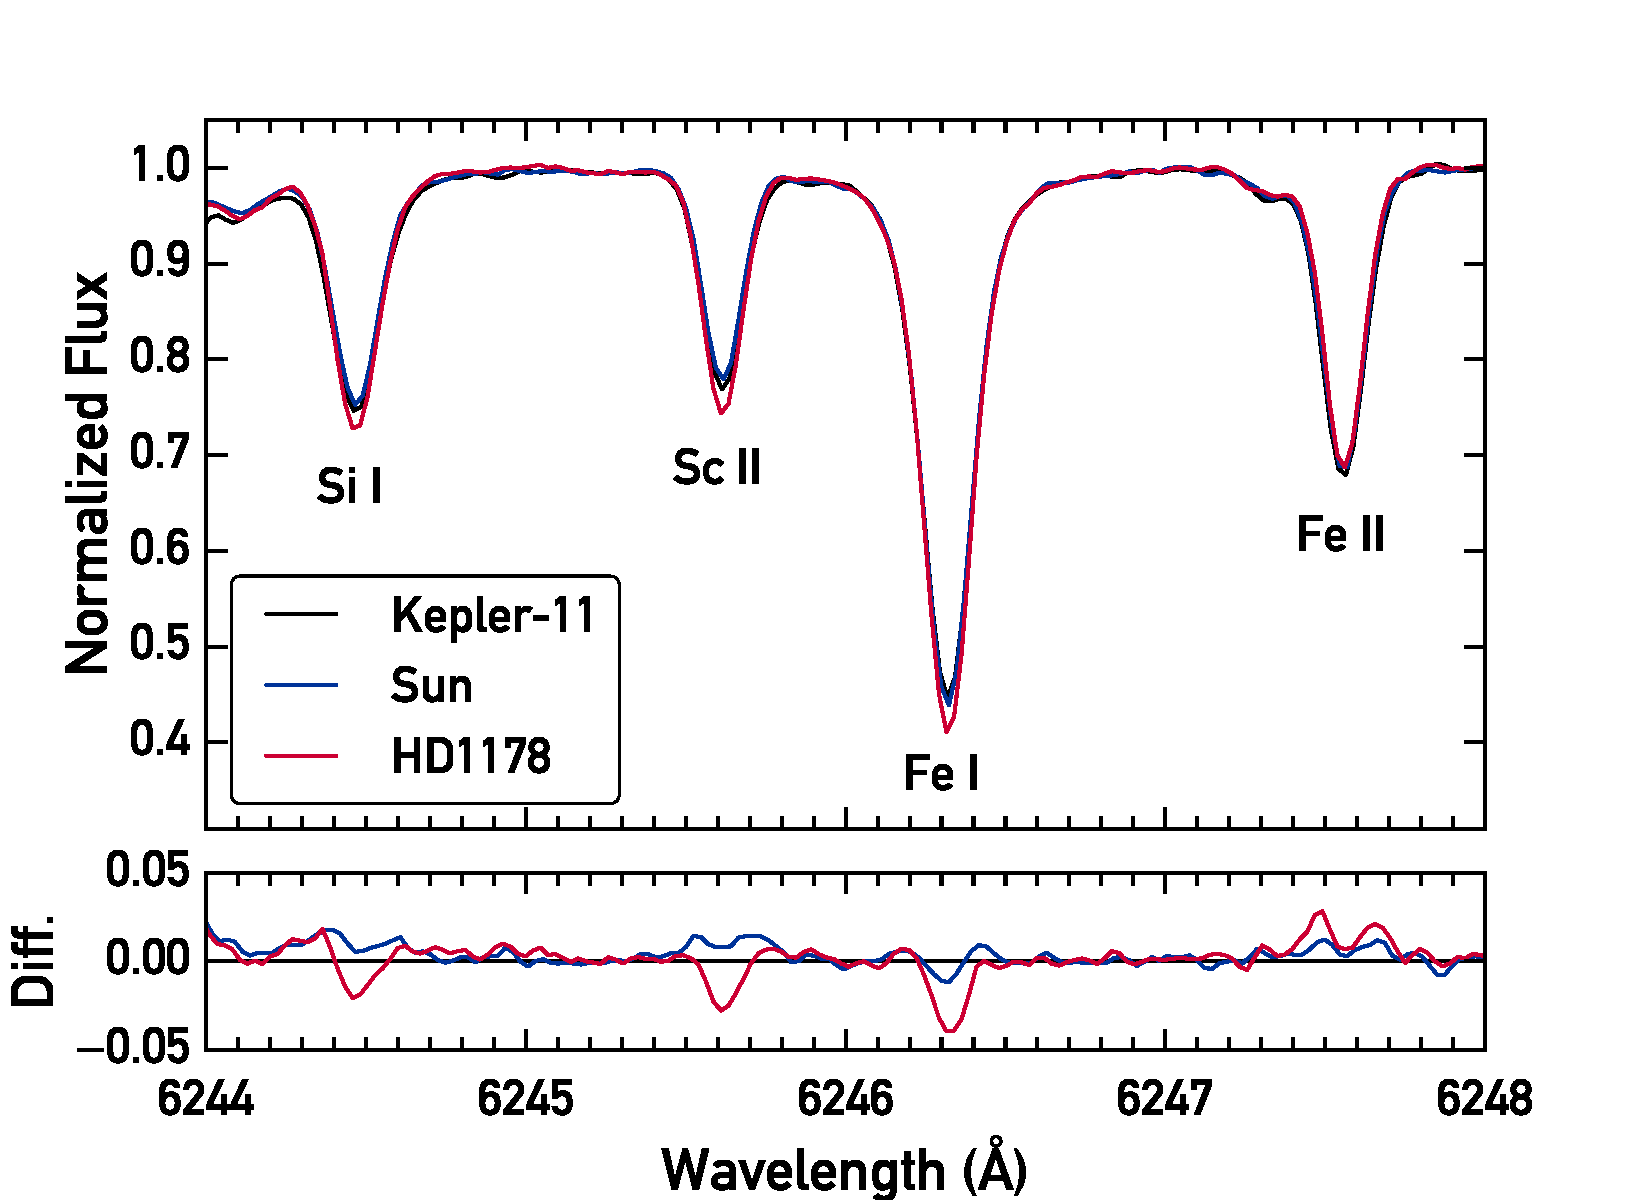
\includegraphics[width=\columnwidth]{spec}
\caption{A small section of the Keck-HIRES spectra of the Sun (blue), Kepler-11 (black), and HD1178 (red), which has fundamental parameters similar to those given by \citet{Lissauer2013} for Kepler-11. Residuals for flux relative to the Kepler-11 spectrum are plotted in the lower panel.}
\label{fig:spec}
\end{figure}

\begin{table*}
\caption{Summary of derived fundamental stellar properties.}
\label{tbl:param}
\centering 
\begin{tabular}{l|cccccccc} 
\hline    
\hline 
{Spectrum}& \teff & $\sigma_{T}$ & \logg & $\sigma_{logg}$ & $v_t$ & $\sigma_{v_t}$ & \feh & $\sigma_{[Fe/H]}$ \\
{}               & (K)           & (K)                 & (dex)     & (dex)                   & (\kms) & (\kms) & (dex) & (dex)  \\
\hline
Sun (Ceres) \footnotemark[1] & 5777 &  & 4.44 &  & 0.97 &   & 0.0 & \\
K11 & 5836 & 7 & 4.44 & 0.02 & 0.98 & 0.02 & 0.062 & 0.007 \\
HD1178 & 5650 & 7 & 4.36 & 0.02 & 0.93 & 0.02 & 0.013 & 0.008 \\
HD10145 & 5637 & 16 & 4.39 & 0.05 & 0.87 & 0.04 & -0.016 & 0.017 \\
HD16623 & 5791 & 26 & 4.37 & 0.07 & 0.97 & 0.06 & -0.462 & 0.022 \\
HD20329 & 5606 & 7 & 4.38 & 0.02 & 0.88 & 0.02 & -0.094 & 0.008 \\
HD21727 & 5618 & 20 & 4.40 & 0.07 & 0.90 & 0.05 & 0.005 & 0.017 \\
HD21774 & 5756 & 29 & 4.32 & 0.07 & 0.98 & 0.06 & 0.252 & 0.026 \\
HD28474 & 5751 & 17 & 4.47 & 0.06 & 0.93 & 0.05 & -0.614 & 0.014 \\
HD176733 & 5609 & 9 & 4.41 & 0.03 & 0.87 & 0.02 & -0.018 & 0.007 \\
HD191069 & 5729 & 30 & 4.29 & 0.09 & 1.01 & 0.07 & -0.033 & 0.025 \\
\hline       
\multicolumn{4}{l}{%
  \begin{minipage}{5.5cm}%
    \footnotetext[1]{Used as reference star.}%
  \end{minipage}%
}\\
\end{tabular}
\end{table*}

\begin{figure}
\centering
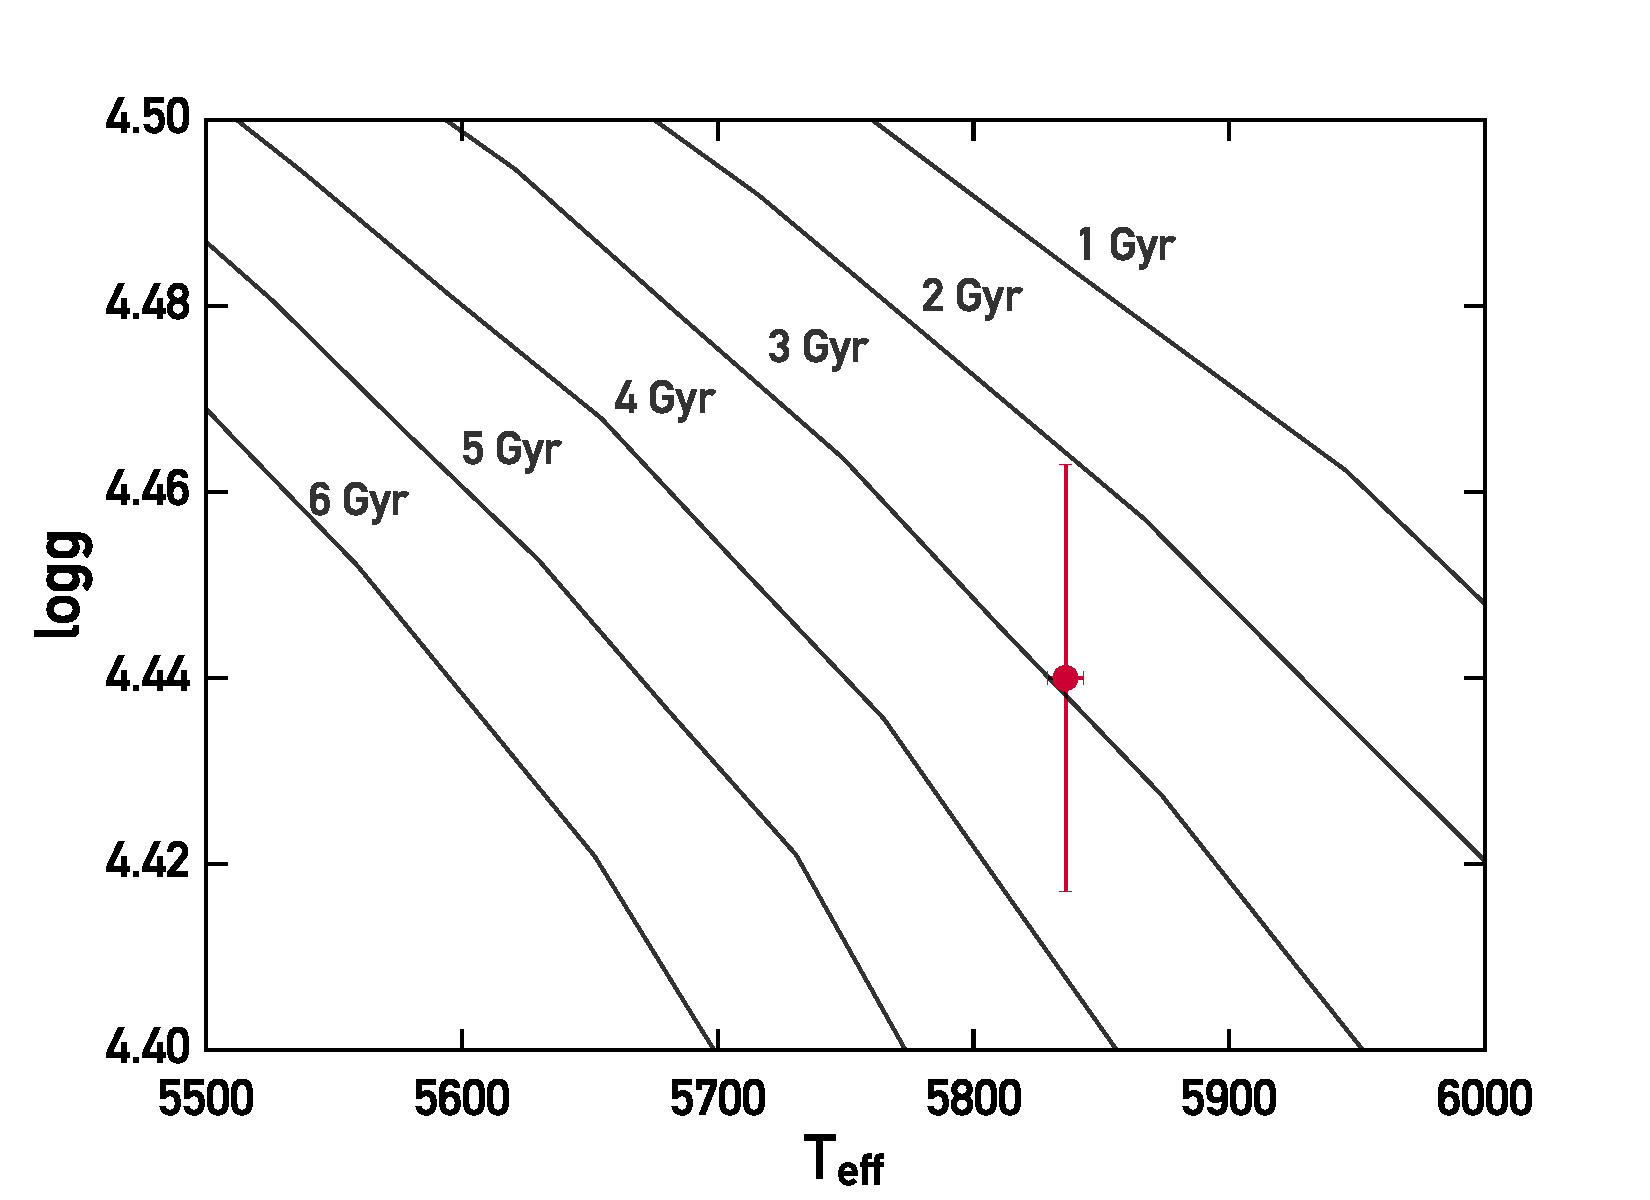
\includegraphics[width=\columnwidth]{isochrones}
\caption{Measured stellar properties of Kepler-11 plotted with Yonsei-Yale isochrones at a metallicity of 0.06 dex.}
\label{fig:isochrones}
\end{figure}

\section{Alternative Stellar Age Indicators}
\label{s:ages}

While mass, radius, and density cannot be measured through methods other than the stellar spectrum, stellar age has multiple known proxies. We used several alternate methods to measure the age of Kepler-11 as an independent test of its evolutionary state. The results unanimously agree upon a sub-solar age for Kepler-11 \todo{(table?)}. Details of the methods used follow.

\subsection{Stellar Rotation}

The apparent rotation rate \vsini\ was measured using five saturated lines (Fe I 6027.050 \r{A}, 6151.618 \r{A}, 6165.360 \r{A}, 6705.102 \r{A}, and Ni I 6767.772 \r{A}) from the Keck spectrum. The procedure used is described in depth in \citet{dosSantos2016}, and will be summarized here. We first measured the macroturbulence value \vmacro$_{,\odot}$\ for each line in the solar reference spectrum using MOOG \textit{synth} with \vsini$_{\odot}$\ fixed at 1.9 \kms. We then calculated \vmacro\ for Kepler-11 using the measured solar values and the empirical relation given in Equation 1 of \citet{dosSantos2016}. Finally, MOOG \textit{synth} was used to find \vsini\ for each line in Kepler-11's spectrum with \vmacro\ fixed to the calculated value.

The five lines give a consistent result of \vsini\ = 2.2 $\pm$ 0.2 \kms. Assuming alignment of the stellar spin axis with the orbital axis of its transiting planets, we can take \vsini\ as the true rotational velocity. \todo{(starspots in LC?)} This translates to an age of 3.4 Gyr using the law of \citet{Skumanich1972} anchored by the Sun, or 3.0 $\pm$ \todo{2.9??} Gyr from \citet{dosSantos2016}'s updated relation.
%Adopting a stellar inclination $i$ = 89.1$^{\circ}$ from \citet{Lissauer2013} and a stellar radius 1.00 \pm$ 0.02 $R_{\odot}$ gives a rotation period of 23 $\pm$ \textbf{x} days.

\subsection{Lithium Abundance}
\label{s:lithium}

The lithium abundance of Kepler-11 was measured by synthesizing the Li I 6707.8 \r{A} line with MOOG \textit{synth}. The line list was adopted from \citet{Melendez2012} and includes blends of atomic and molecular lines. We find a lithium abundance of \textit{A}(Li) = 1.26 $\pm$ 0.05, higher than the solar value of 1.11 at the level of 3$\sigma$ (Figure \ref{fig:lithium}). This implies a sub-solar age, since lithium is steadily depleted throughout a star's main-sequence lifetime \todo{(cite)}.

\begin{figure}
\centering
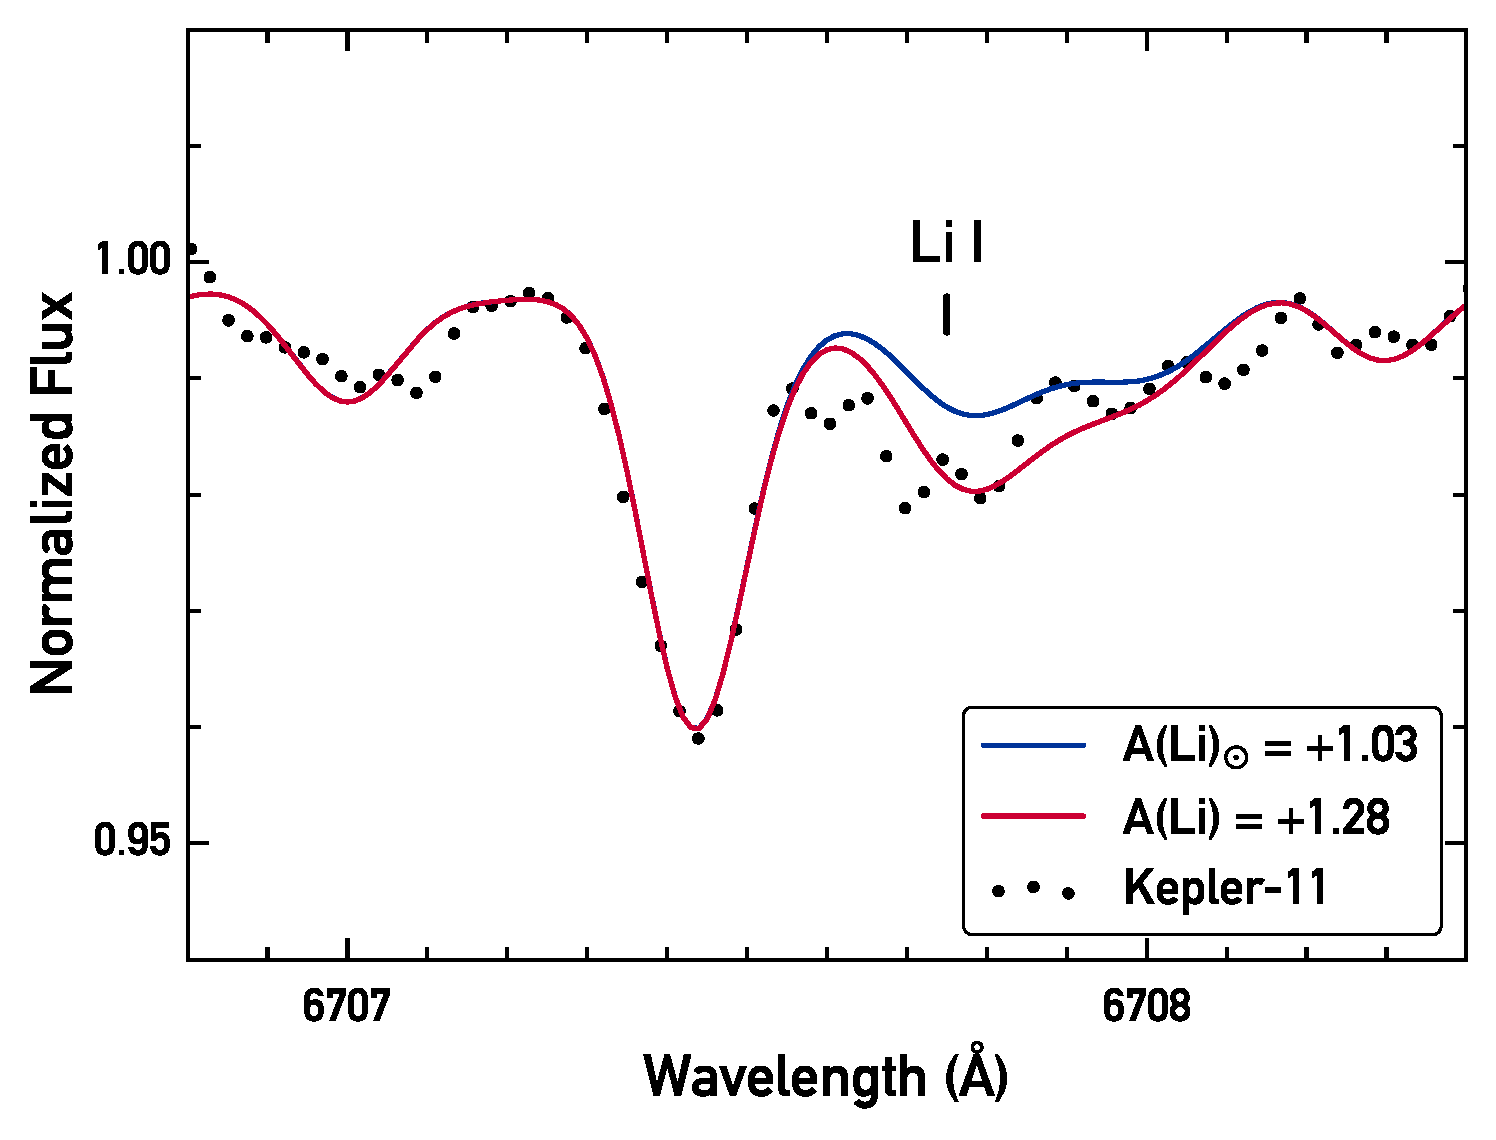
\includegraphics[width=\columnwidth]{lithium}
\caption{Observed spectrum of Kepler-11 around the Li I 6707.8 \r{A} line. Synthetic fits for the best-fit Li abundance (red) and the solar Li abundance (blue) are overplotted. \todo{(fix up this fit!)}}
\label{fig:lithium}
\end{figure}


\subsection{[Y/Mg] Abundance Ratio}

Recent works by \citet{Nissen2015} and \citet{TucciMaia2016} have identified the ratio of yttrium to magnesium abundances as an excellent proxy for age in main-sequence Sun-like stars. We measured these abundances as described in Section \ref{s:abundances} and found a [Y/Mg] ratio of 0.04 $\pm$ 0.05 dex. Using the age relation from \citet{TucciMaia2016}, this gives an age of 4.0 $\pm$ 0.7 Gyr. \todo{double-check these numbers}

\subsection{Chromospheric Emission}

We measured the chromospheric emission level of Kepler-11 using the Ca II H line. Since our spectral coverage cut off around 390 nm at the blue end, it was not possible to obtain a measurement of the standard chromospheric activity index $\log(\mathrm{R'_{HK}})$. Instead, we defined an alternative index \textit{H} as the flux integrated from a 1.3 \r{A} width triangular filter centered on the H line at 3968.47 \r{A}, divided by the continuum integrated with a flat filter of 5 \r{A} width around 3979.8 \r{A}.  \todo{conversion details}

We find an activity index $\log(\mathrm{R'_{HK}})$ = -4.78. This is slightly higher than the maximum activity level of the solar cycle and suggests a sub-solar age \citep{Hall2009, Ramirez2014}.


\section{Stellar Abundances}
\label{s:abundances}

We measured photospheric abundances using the curve-of-growth technique for 20 other elements (excluding lithium, whose synthesis-based abundance determination is discussed in Section \ref{s:lithium}). As with the iron lines, all equivalent widths were measured by hand and line-by-line differential abundances determined with MOOG using $q^2$. The line list was adapted from previous works including \citet{Bedell2014}. Hyperfine structure corrections were applied for Co I, Cu I, Mn I, V I, and Y II following \todo{(cite)}. Carbon abundances were measured by a combination of C I and CH lines. Errors on the final abundances were found by adding in quadrature the intrinsic scatter of the lines and the uncertainty propagated from errors on the stellar parameters. The measured equivalent widths are given in Table \ref{tbl:ews}, and resulting abundances for all stars are in Table \ref{tbl:abund}.

Kepler-11's status as a solar twin enables direct comparison of its abundance pattern to that of the Sun and other known solar twins. Of particular interest is the question of trends in elemental abundances with condensation temperature (\tc). As shown by \citet{Melendez2009}, the solar abundance pattern is unusual in its depletion of refractory elements relative to volatiles. This depletion has been interpreted as ``missing'' rocky material that is locked up in the Solar System planets \citep{Chambers2010}. Building up the number of stars with precisely characterized abundance patterns and planetary systems can help to test this possibility.

We apply corrections for the effects of galactic chemical evolution (GCE), which can change the abundance patterns and \tc\ trends of stars at varying ages \citep{Nissen2015, Spina2016}. We correct each abundance [X/H] using the prescription of \citet{Spina2016b}, who fit hyperbolic relations to [X/H] as a function of stellar age for a sample of solar twins. We then use the corrected abundances and \tc\ values from Table 8 of \citet{Lodders2003} to search for a trend. For this part of the analysis, all measured states of a given element (e.g. CI and CH, TiI and TiII, etc.) were combined with a weighted average for the overall elemental abundance. %Although we use differential abundances relative to iron for the fit to be consistent with past literature, we note that the uncertainties used actually correspond to the error on [X/H] rather than [X/Fe]. As noted by \citet{Adibekyan2016}, propagating the iron abundance uncertainty would effectively even out the weighting used in the \tc\ trend fit. This would be inaccurate since any error in the iron abundance will, to first order, shift all points equally and have no effect on the slope of the \tc\ trend.

Based on our analysis, Kepler-11 appears to be a ``typical'' solar twin: that is, its abundance pattern is enhanced in refractories relative to the solar pattern (Figure \ref{fig:tc}). The significance of this enhancement depends on the stellar age adopted for the GCE correction. Without GCE correction applied, the \tc\ slope is significant only at the 2$\sigma$ level, whereas adopting an age of 2.8 Gyr enhances the slope to above 3$\sigma$.

\todo{(Adjust Tc figure \& discussion to use bootstrapped errors on slope.)}

\begin{figure*}
\centering
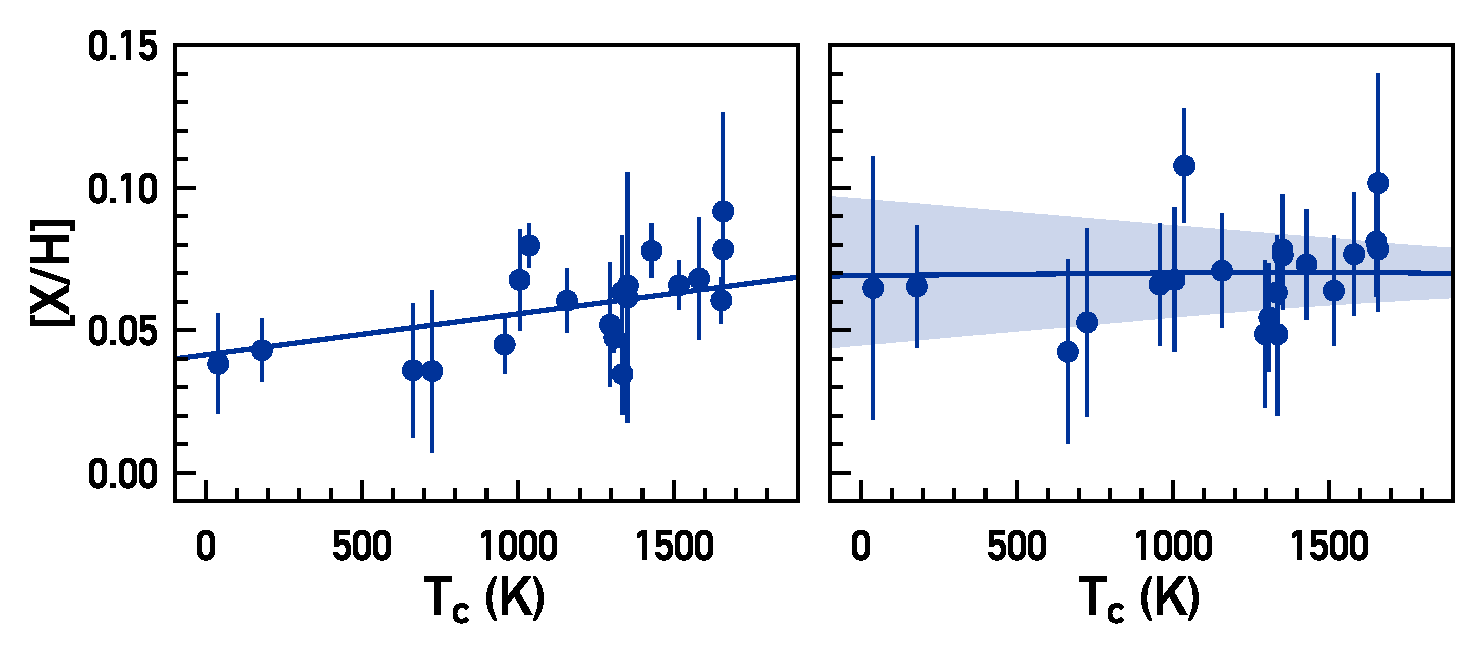
\includegraphics[scale=0.45]{K11_Tc_linear}
\caption{Abundances of Kepler-11 relative to the Sun as a function of the condensation temperature of the element within the protoplanetary disk. The spectral abundances are plotted in blue, and abundances after a GCE correction is applied are in red. Note that the uncertainties increase after GCE correction due to the propagated uncertainty in the correction factors and in the stellar age. \todo{(add in a legend with slope values and errors)}}
\label{fig:tc}
\end{figure*}




\section{Stellar Properties from Photodynamic Transit Analysis}
\label{s:ttvs}

In order to reassess the stellar density constraint based on the transit data, we performed a photodynamical fit to the full \Kepler short cadence (58.8 second exposure) data set. The model integrates the 7-body Newtonian equations of motions for the central star and two planets, including the light--travel--time effect. When the planets pass between the star and the line of sight, a synthetic light curve is generated \citep{2012MNRAS.420.1630P}, which can then be compared to the data. This approach therefore takes into account all transit-timing variations and can constrain planet masses and eccentricities as well as radii. To prepare the data for fitting, we detrended the data with a cubic polynomial with a 2880 minute (2 day) width every 100 points, and interpolated for points between. We divide the flux by this fit as a baseline to generate our data set of 1746779 points. We additionally multiply the uncertainties given by \Kepler by a factor of 1.115318 so that the reduced $\chi^2$ of a fiducial model was 1.0. This will broaden our posteriors and helps take into account unmodeled noise in the data. To simultaneously generate the posteriors on all of our model parameters, we ran differential evolution Markov chain Monte Carlo \cite[DEMCMC, ][]{TerBraak2005} fits with planetary parameters $\{P,\, T_0,\, e^{1/2} \, \cos(\omega),\, e^{1/2} \, \sin(\omega),\, i,\, \Omega,\, R_\mathrm{p}/R_\star,\, M_\mathrm{p}/M_\star\}$ for all planets, where $P$ is the period, $T_0$ is the mid-transit time, $e$ is eccentricity, $\omega$ is the argument of periapse, $i$ is inclination, $\Omega$ is nodal angle, and $R$ and $M$ are radius and mass respectively (with subscripts p $=$ b, c, d, e, f, g for the planets and $\star$ for the star). The star had five additional parameters: $\{M_\star,\, R_\star,\, c_1,\, c_2,\, dilute\}$, where $\{c_i\}$ are the two quadratic limb-darkening coefficients and $dilute$ is the amount of dilution from other nearby sources. We use eccentricity vector components scaling as $e^{1/2}$ so that we have flat prior in total $e$, and fix the values of $dilute=0$ since there is no evidence of other nearby stars diluting the lightcurve. We also fix the value of $M_\star$ as transits alone generally only give information about the density of the star, rather than $M_\star$ and $R_\star$ individually. We fix $\Omega = 0$ for all planets because the data is not precise enough to constrain these values \citep{Migaszewski2012}. Additionally, it is extremely unlikely that there are large mutual inclinations among the planets given that we see six planets transit (L11, Figure 4), five of which are dynamically packed and thus have no misaligned non-transiting planets between them (L11). We use flat priors in all other parameters.

We run two DEMCMCs. One has no constraints on the stellar radius, i.e., allows the transits themselves to completely determine the stellar density, which we will label $\mathcal{NSI}$, for No Spectral Information. The second DEMCMC we run with the stellar mass and radius fixed at the spectroscopically measured values in this study, $M_\star=1.04M_\odot$ and $R_\star=1.00M_\odot$, which we will label $\mathcal{FSP}$, for Fixed Stellar Parameters. The $\mathcal{NSI}$ run produces a lower density star $\rho_\star = 1.191^{+0.043}_{-0.11}$ g cm$^{-3}$ than the fixed value of $\rho_\star = 1.466$ g cm$^{-3}$ in $\mathcal{FSP}$. This indicates that the transit data alone are discrepant with the spectroscopically measured stellar density. Table~\ref{table:den} shows the density results for all bodies for both DEMCMC runs. We note that the densities of planets with no spectral information, $\mathcal{NSI}$, are slightly higher than reported in L13 because that study includes the lower spectroscopically measured stellar density in their final best fits.

The best fit solution from $\mathcal{NSI}$ run has $\chi^2 = 1746731$, while the $\mathcal{FSP}$ run has $\chi^2 = 1746778$, a difference of 47. Thus we see that fixing the stellar parameters at their spectroscopically measured values causes the fit to the \Kepler data to become statistically significantly worse since there is only one more degree of freedom (stellar density) in the $\mathcal{NSI}$ model than the $\mathcal{FSP}$ model. This confirms the existence of tension between the transit measured stellar density and the spectroscopically measured one.  

\begin{table}
\caption{Star and Planet Densities}
\label{table:den}
\centering 
\begin{tabular}{l c c} 
\hline
Body & $\mathcal{NSI}$ & $\mathcal{FSP}$  \\
 & Density (g cm$^{-3}$)  & Density (g cm$^{-3}$) \\
\hline
Kepler-11    & $1.191^{+0.043}_{-0.11} $& $1.466 $ (fixed) \\
Kepler-11 b & $2.43^{+0.64}_{-0.61} $ & $ 3.14^{+0.71}_{-0.76} $  \\
Kepler-11 c &  $ 1.09^{+0.31}_{-0.31} $ &$ 1.41^{+0.35}_{-0.40} $ \\
Kepler-11 d &  $ 1.32^{+0.14}_{-0.15} $ & $ 1.53^{+0.13}_{-0.14} $ \\
Kepler-11 e &  $ 0.657^{+0.076}_{-0.080} $ & $ 0.749^{+0.092}_{-0.093} $ \\
Kepler-11 f &  $ 0.82^{+0.17}_{-0.15} $  &$ 0.67^{+0.24}_{-0.23} $  \\
Kepler-11 g &  $ <  4 $ & $ < 5 $\\
\hline       
\end{tabular}
\tablecomments{Medians and 1-$\sigma$ uncertainties from the DEMCMC runs as described in \S~\ref{s:ttvs}}

\end{table}



\begin{figure}
\centering
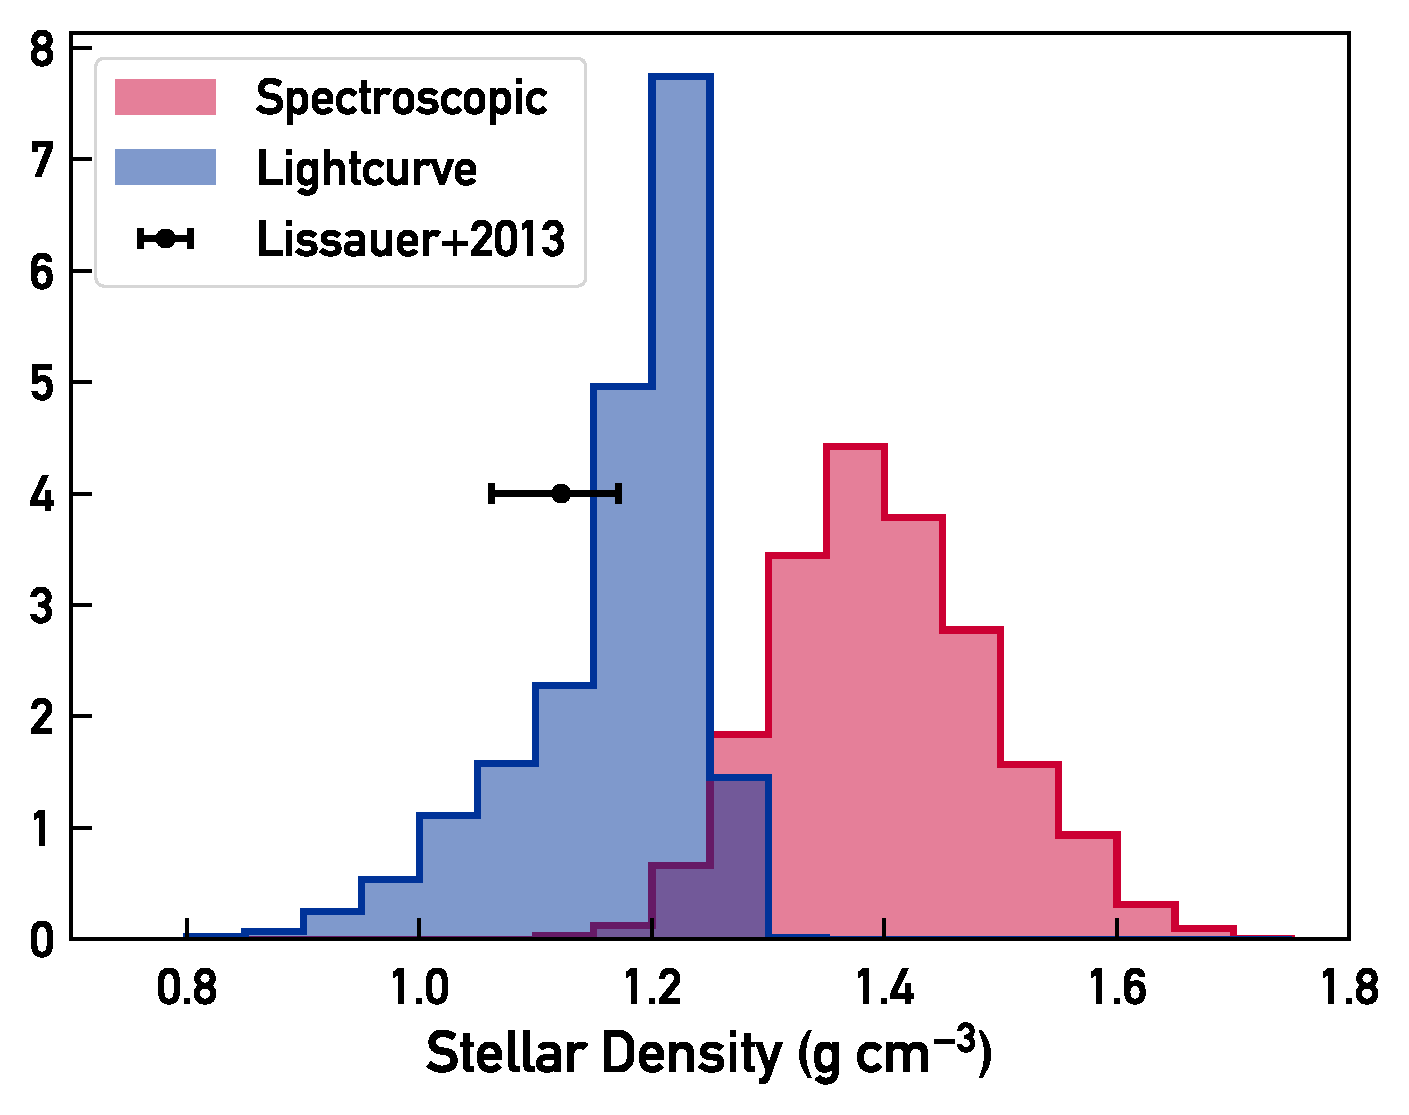
\includegraphics[width=\columnwidth]{density}
\caption{Posterior distributions for the stellar density from isochrone fits to the spectroscopic parameters (red) and from photodynamical modeling of the lightcurve (blue).}
\label{fig:densities}
\end{figure}


\section{Discussion}
\label{s:discussion}
\subsection{Discrepancies in Stellar Densities}

The stellar densities found through spectroscopic characterization (1.47 $\pm$ 0.09 \gcm) and photodynamical modeling (1.13 $\pm$ 0.07 \gcm) are inconsistent at the level of $\sim$3$\sigma$ \todo{(is this true anymore? why did it change?)} (Figure \ref{fig:densities}). While spectroscopically-derived densities can be strongly dependent on imperfect stellar isochrone models, we note that in this case Kepler-11's extreme similarity to the Sun places it near the anchor point of most models, increasing the accuracy of isochronal analysis. Moreover, multiple independent methods support the result of a young, non-evolved age and therefore a solar-like density for Kepler-11.

An alternative hypothesis is that some bias in the transit analysis has resulted in an erroneously low inferred stellar density. As described by \citet{Kipping2014}, multiple effects can bias the density measured by transits, including stellar activity, blended background sources, and non-zero planet eccentricities. Bias due to an underestimated planet eccentricity is not a likely explanation in this case, since all five planets give a consistent stellar density. Also, the photodynamical modeling used in this analysis should be robust to the effects of transit timing or duration variations on the measured stellar density. This leaves two potentially viable explanations from \citet{Kipping2014} for the density discrepancy: stellar activity (the ``photospot'' effect) or a background source (the ``photoblend'' effect).

Starspots effectively reduce the observed stellar flux, artificially raising stellar density inferred from the transit depth, which is the opposite of the effect we seek to explain. However, as a middle-aged Sun-like star, Kepler-11's activity may manifest mostly in the form of plages \todo{(cite)}. Unocculted plages could potentially lower the observed stellar density. Given the observed behavior of other main-sequence solar analogs and the lack of rotational modulation in the \Kepler lightcurve, the filling factor for spots or plages on Kepler-11's surface should be of order 1\% \todo{(cite)}. This would yield a similarly small change in the observed stellar density \citep[O($10^{-2}$),][]{Kipping2014}. Furthermore, the plage configuration would need to be relatively stable throughout \Kepler's four years of observations, since the transit depths do not noticeably change with time \todo{(check with Sean on this)}, which is unlikely at the high level of activity needed to have a filling factor $\gg$ 1\%.

The final effect is blending of unresolved background sources, which can cause stellar density to be underestimated. Recently \citet{Wang2015} found two visual companions to Kepler-11 at separations of 1.36'' and 4.9'' using AO imaging, both potentially within Kepler's resolution. With brightness differences of $\Delta K$ = 4.4 mag and 4.7 mag respectively, these companions should contribute approximately 3\% of the total flux in the Kepler bandpass \todo{(true?)}. Using Equation 9 of \citet{Kipping2014}, this implies that the observed stellar density from transits should be $\sim$99\% of the true density. The known companions are therefore insufficient to explain the magnitude of the density discrepancy.

\todo{so....?}

\subsection{Implications for the Planets}

The mass and radius of Kepler-11 has considerable repercussions for its planetary system. We approximate the planet mass derived from TTVs as a linear function of the assumed stellar mass. The planet radius also has a linear dependence on stellar radius, since only the relative surface areas of planet and star can be measured by the transit depth. The stellar properties obtained through spectroscopic analysis therefore raise the planet masses by a factor of 8\% and lower the planet radii by a factor of 6\% relative to the transit and TTV-derived values. The results are shown in Figure \ref{fig:mr}.

Adopting the stellar properties from spectroscopic analysis raises the mean densities of the Kepler-11 planets by $\sim$30\%. This change may go a long way in resolving the lingering debate over the viability of in-situ formation of these planets. \todo{(finish - talk to Leslie?)}

\subsection{Stellar Composition \& Planets}

Kepler-11's photospheric abundances are likely... \todo{compare to Kepler-10, Sun}

The relatively large uncertainty on the condensation temperature trend underscores the importance of galactic chemical evolution effects. Although we have achieved very high-precision stellar abundance measurements, more work remains to be done on disentangling potential planet formation signatures from other effects. For an individual system, even a solar twin with an age within a couple Gyr of the Sun, the uncertain effects of GCE make it extremely challenging to draw conclusions about the significance of the stellar abundance pattern in the context of planet formation. Fortunately, large-scale surveys like APOGEE and GAIA-ESO will provide the large sample sizes needed to refine high-precision abundance-age relations.

\begin{figure*}
\centering
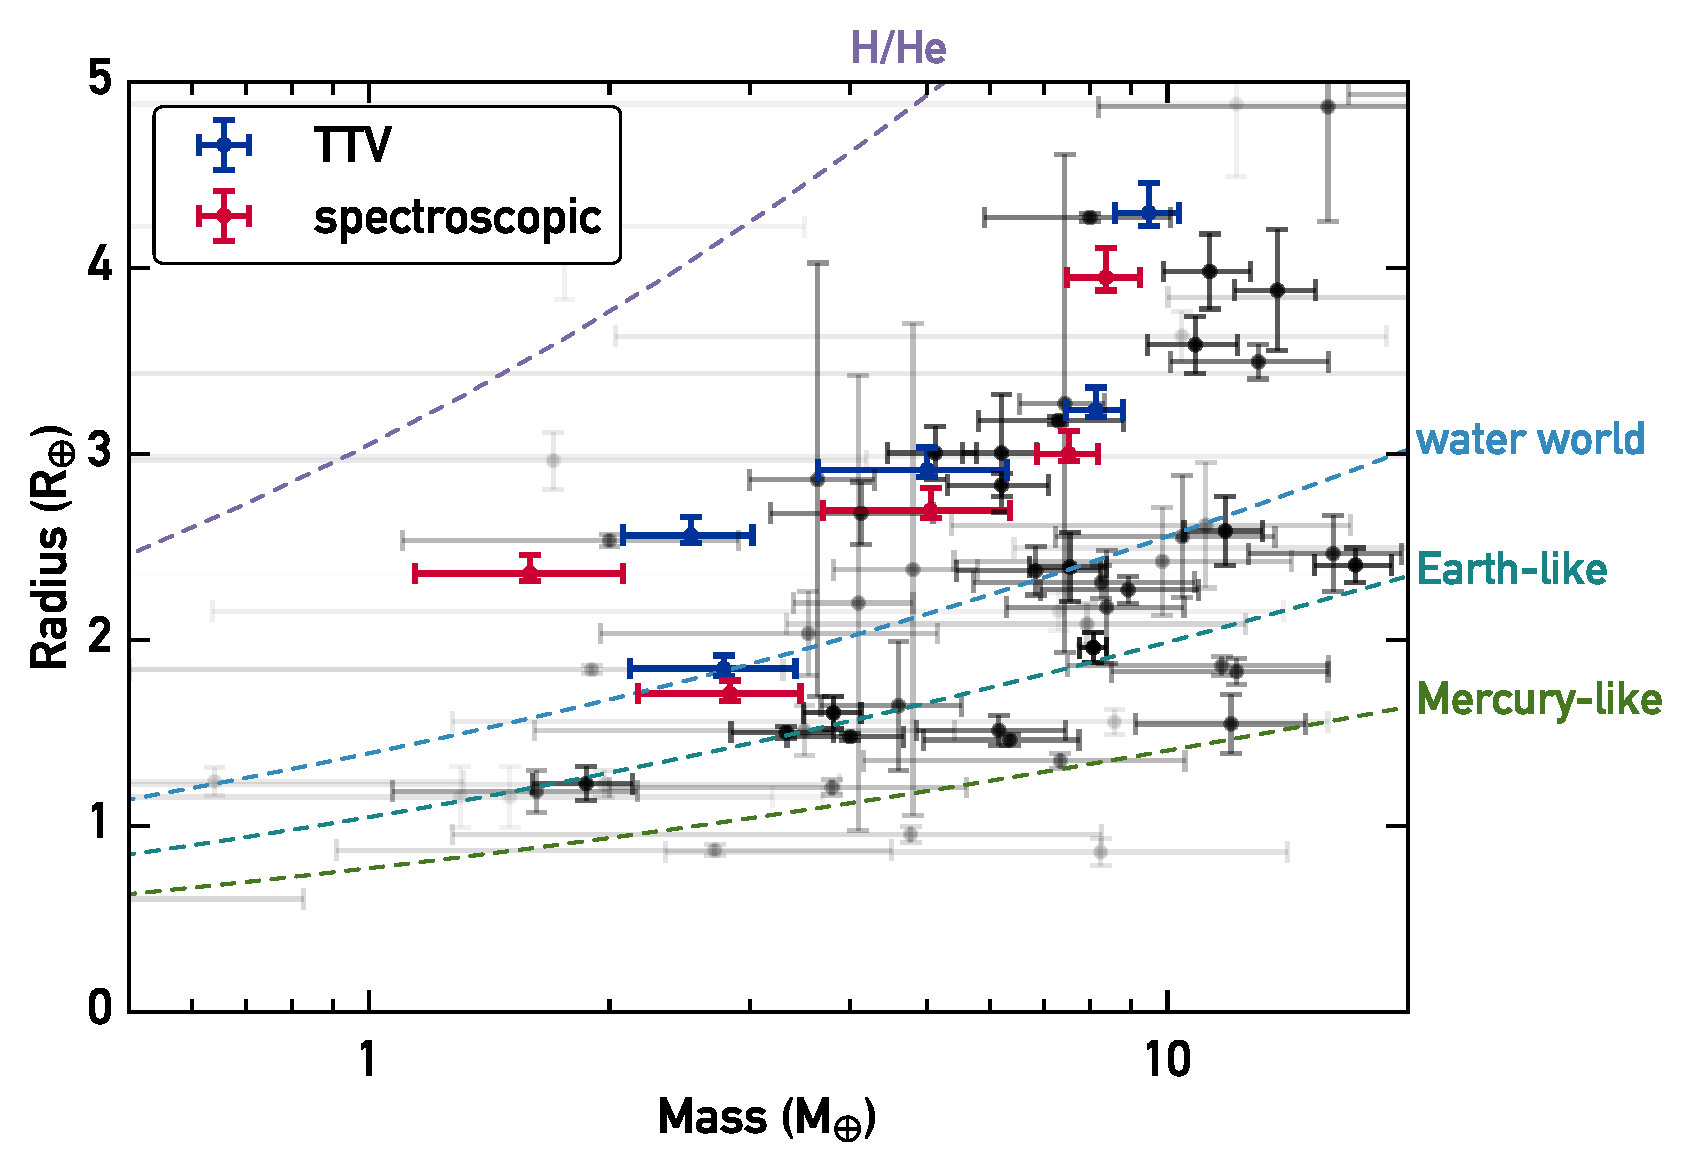
\includegraphics[scale=0.6]{K11_massradius}
\caption{Exoplanets with measured masses and radii. Transparencies of the black points scale with the relative error on planet parameters. Kepler-11 a-e are plotted in red (using the transit and TTV-derived parameters) and blue (adjusted by the spectroscopic stellar parameters). Dashed lines show fixed mean densities.}
\label{fig:mr}
\end{figure*}


\section{Conclusion}

Using an extremely high-quality spectrum of the multi-planet host star Kepler-11, we have measured the stellar fundamental parameters and abundances to percent-level precision. We have also used a photodynamical model to fit the full \Kepler lightcurve. Our planet parameters agree with past publications. However, we find that the host star is younger than previously thought by a factor of $\sim$3. Based on spectroscopic results, Kepler-11 and its planets are $\sim$30\% denser than previously reported.

The five inner planets of the Kepler-11 system are key members of the exoplanet mass-radius diagram as examples of the surprisingly low densities found in some planetary systems. The substantial revision of their properties reported here underscores the importance of detailed host star follow-up. As the community looks to exponentially increase the number of exoplanets with measured bulk densities through TESS and beyond, it is critical to prioritize securing high-quality spectra of the host stars to enable the determination of precise host star properties.

\bigskip
\acknowledgements{M.B. is supported by a National Science Foundation Graduate Research Fellowship under Grant No. DGE-1144082.  J.L.B. acknowledges support for this work from the NSF (grant number AST-1313119) and the Alfred P. Sloan Foundation.  J.M. thanks FAPESP (2012/24392-2). \todo{update \& finish}}

{\it Facilities:} \facility{Keck:I (HIRES)}, \facility{Kepler}


\bibliographystyle{apj}
\bibliography{K11.bib}

\pagebreak
\begin{sidewaystable}
\caption{Line List and Measured Equivalent Widths.}
\label{tbl:ews}
\centering 
\begin{tabular}{ccccccccccccccc} 
\hline
\hline
{Wavelength} & Species & EP & log($gf$) & Kepler-11 & Sun & HD1178 & HD10145 & HD16623 & HD20329 & HD21727 & HD21774 & HD28474 & HD176733 & HD191069 \\
 (\r{A}) &  & (eV) & (dex) & (m\r{A}) & (m\r{A}) & (m\r{A}) & (m\r{A}) & (m\r{A}) & (m\r{A}) & (m\r{A}) & (m\r{A}) & (m\r{A}) & (m\r{A}) & (m\r{A}) \\
\hline
5052.167 & 6  & 7.685 & -1.24 & 35.2 & 33.5 & 32.7 & 27.9 & 21.4 & 29.4 & 26.6 & 41.6 & 17 & 27.4 & 36.7 \\
6587.61 & 6 & 8.537 & -1.05 & 16.9 & 15.2 & 17 & 12.2 & 9.8 & 11.4 & 11.7 & 20.3 & 6.2 & 10.8 & 17 \\
7111.47 & 6 & 8.64 & -1.07 & 13.2 & 11.3 & 12.1 & 15.1 & 9.6 & 12.3 & 10.9 & 16.6 & 36.7 & 10.2 & 14 \\
7113.179 &  6 & 8.647 & -0.76 & 25.3 & 22.4 & 23.2 & 20.3 & 13.8 & 17.9 & 19.5 & 33 & 11.3 & 18.2 & 24.3 \\
7771.944 & 8 & 9.146 & 0.37 & 77.8 & 69.7 & 79.1 & 63.6 & 71 & 69.4 & 62.9 & 79.9 & 56.9 & 61.5 & 81.8 \\
  &  & & & & & & $\vdots$   & &  & & & & \\
\hline       
\end{tabular}
\tablecomments{Table \ref{tbl:ews} is published in its entirety in the electronic edition of ApJ. A portion is shown here for guidance regarding its form and content.}


\end{sidewaystable}


\pagebreak


\begin{sidewaystable}
\caption{Differential Abundances [X/H].}
\label{tbl:abund}
%\centering 
\begin{tabular}{lccccccccccc} 
\hline    
\hline 
{Element} & $N_{lines}$ & Kepler-11 & HD1178 & HD10145 & HD16623 & HD20329 & HD21727 & HD21774 & HD28474 & HD176733 & HD191069 \\
\hline
CI & 4 & 0.03 $\pm$ 0.01 & 0.12 $\pm$ 0.04 & 0.07 $\pm$ 0.12 & -0.20 $\pm$ 0.08 & 0.05 $\pm$ 0.08 & 0.03 $\pm$ 0.06 & 0.18 $\pm$ 0.04 & -0.09 $\pm$ 0.46 & 0.01 $\pm$ 0.05 & 0.07 $\pm$ 0.03 \\
OI & 3 & 0.06 $\pm$ 0.01 & 0.18 $\pm$ 0.08 & 0.08 $\pm$ 0.02 & -0.09 $\pm$ 0.02 & 0.17 $\pm$ 0.03 & 0.08 $\pm$ 0.03 & 0.20 $\pm$ 0.02 & -0.27 $\pm$ 0.02 & 0.05 $\pm$ 0.03 & 0.14 $\pm$ 0.02 \\
NaI & 4 & 0.04 $\pm$ 0.02 & -0.03 $\pm$ 0.02 & -0.12 $\pm$ 0.05 & -0.39 $\pm$ 0.02 & -0.04 $\pm$ 0.04 & -0.08 $\pm$ 0.03 & 0.27 $\pm$ 0.03 & -0.56 $\pm$ 0.05 & -0.03 $\pm$ 0.03 & -0.01 $\pm$ 0.02 \\
MgI & 5 & 0.04 $\pm$ 0.03 & 0.10 $\pm$ 0.03 & 0.05 $\pm$ 0.01 & -0.23 $\pm$ 0.05 & 0.05 $\pm$ 0.12 & 0.06 $\pm$ 0.06 & 0.26 $\pm$ 0.04 & -0.41 $\pm$ 0.06 & 0.03 $\pm$ 0.04 & 0.09 $\pm$ 0.02 \\
AlI & 2 & 0.06 $\pm$ 0.01 & 0.18 $\pm$ 0.02 & 0.04 $\pm$ 0.01 & -0.30 $\pm$ 0.01 & 0.18 $\pm$ 0.03 & 0.07 $\pm$ 0.01 & 0.28 $\pm$ 0.01 & -0.47 $\pm$ 0.01 & 0.04 $\pm$ 0.01 & 0.11 $\pm$ 0.01 \\
SiI & 14 & 0.05 $\pm$ 0.02 & 0.04 $\pm$ 0.03 & 0.00 $\pm$ 0.01 & -0.28 $\pm$ 0.03 & 0.04 $\pm$ 0.05 & 0.02 $\pm$ 0.03 & 0.24 $\pm$ 0.02 & -0.46 $\pm$ 0.04 & -0.00 $\pm$ 0.02 & 0.04 $\pm$ 0.01 \\
SI & 4 & 0.04 $\pm$ 0.04 & 0.11 $\pm$ 0.04 & 0.06 $\pm$ 0.03 & -0.25 $\pm$ 0.06 & 0.03 $\pm$ 0.09 & 0.02 $\pm$ 0.03 & 0.23 $\pm$ 0.03 & -0.39 $\pm$ 0.09 & 0.03 $\pm$ 0.05 & 0.09 $\pm$ 0.05 \\
KI & 1 & 0.08 $\pm$ 0.00 & 0.03 $\pm$ 0.00 & -0.03 $\pm$ 0.00 & -0.17 $\pm$ 0.00 & -0.02 $\pm$ 0.00 & -0.06 $\pm$ 0.00 & 0.20 $\pm$ 0.00 & -0.35 $\pm$ 0.00 & -0.06 $\pm$ 0.00 & 0.07 $\pm$ 0.00 \\
CaI & 11 & 0.07 $\pm$ 0.02 & 0.07 $\pm$ 0.03 & 0.02 $\pm$ 0.01 & -0.30 $\pm$ 0.02 & 0.05 $\pm$ 0.04 & 0.04 $\pm$ 0.03 & 0.23 $\pm$ 0.02 & -0.49 $\pm$ 0.02 & -0.00 $\pm$ 0.02 & 0.03 $\pm$ 0.01 \\
ScI & 4 & 0.09 $\pm$ 0.04 & 0.10 $\pm$ 0.03 & 0.03 $\pm$ 0.03 & -0.34 $\pm$ 0.06 & 0.07 $\pm$ 0.06 & 0.04 $\pm$ 0.03 & 0.27 $\pm$ 0.03 & -0.37 $\pm$ 0.08 & 0.01 $\pm$ 0.04 & 0.07 $\pm$ 0.01 \\
ScII & 5 & 0.10 $\pm$ 0.02 & 0.14 $\pm$ 0.05 & 0.04 $\pm$ 0.01 & -0.29 $\pm$ 0.04 & 0.14 $\pm$ 0.05 & 0.11 $\pm$ 0.05 & 0.32 $\pm$ 0.02 & -0.47 $\pm$ 0.04 & 0.00 $\pm$ 0.01 & 0.12 $\pm$ 0.04 \\
TiI & 18 & 0.07 $\pm$ 0.02 & 0.11 $\pm$ 0.02 & 0.05 $\pm$ 0.04 & -0.24 $\pm$ 0.03 & 0.15 $\pm$ 0.03 & 0.06 $\pm$ 0.03 & 0.24 $\pm$ 0.04 & -0.45 $\pm$ 0.02 & 0.01 $\pm$ 0.02 & 0.08 $\pm$ 0.02 \\
TiII & 11 & 0.07 $\pm$ 0.03 & 0.11 $\pm$ 0.05 & 0.02 $\pm$ 0.09 & -0.23 $\pm$ 0.05 & 0.12 $\pm$ 0.03 & 0.03 $\pm$ 0.10 & 0.26 $\pm$ 0.04 & -0.42 $\pm$ 0.03 & -0.01 $\pm$ 0.03 & 0.10 $\pm$ 0.04 \\
VI & 9 & 0.08 $\pm$ 0.02 & 0.08 $\pm$ 0.02 & -0.01 $\pm$ 0.02 & -0.32 $\pm$ 0.03 & 0.10 $\pm$ 0.09 & 0.04 $\pm$ 0.03 & 0.28 $\pm$ 0.02 & -0.53 $\pm$ 0.04 & 0.01 $\pm$ 0.02 & 0.03 $\pm$ 0.02 \\
CrI & 10 & 0.05 $\pm$ 0.02 & 0.02 $\pm$ 0.02 & 0.01 $\pm$ 0.06 & -0.48 $\pm$ 0.04 & -0.07 $\pm$ 0.03 & 0.01 $\pm$ 0.02 & 0.27 $\pm$ 0.04 & -0.63 $\pm$ 0.06 & 0.00 $\pm$ 0.02 & -0.02 $\pm$ 0.02 \\
CrII & 5 & 0.06 $\pm$ 0.02 & 0.01 $\pm$ 0.02 & -0.01 $\pm$ 0.05 & -0.41 $\pm$ 0.05 & -0.07 $\pm$ 0.02 & 0.01 $\pm$ 0.03 & 0.24 $\pm$ 0.03 & -0.59 $\pm$ 0.05 & -0.03 $\pm$ 0.02 & -0.03 $\pm$ 0.02 \\
MnI & 8 & 0.06 $\pm$ 0.03 & -0.05 $\pm$ 0.03 & -0.07 $\pm$ 0.03 & -0.63 $\pm$ 0.03 & -0.18 $\pm$ 0.02 & -0.04 $\pm$ 0.02 & 0.30 $\pm$ 0.03 & -0.78 $\pm$ 0.06 & -0.03 $\pm$ 0.02 & -0.08 $\pm$ 0.02 \\
FeI & 92 & 0.06 $\pm$ 0.02 & 0.01 $\pm$ 0.02 & -0.02 $\pm$ 0.05 & -0.46 $\pm$ 0.06 & -0.09 $\pm$ 0.02 & 0.01 $\pm$ 0.07 & 0.25 $\pm$ 0.08 & -0.61 $\pm$ 0.05 & -0.02 $\pm$ 0.03 & -0.03 $\pm$ 0.09 \\
FeII & 17 & 0.06 $\pm$ 0.02 & 0.01 $\pm$ 0.05 & -0.02 $\pm$ 0.11 & -0.46 $\pm$ 0.07 & -0.10 $\pm$ 0.05 & 0.01 $\pm$ 0.03 & 0.25 $\pm$ 0.03 & -0.62 $\pm$ 0.07 & -0.02 $\pm$ 0.02 & -0.03 $\pm$ 0.04 \\
CoI & 6 & 0.06 $\pm$ 0.01 & 0.05 $\pm$ 0.04 & -0.03 $\pm$ 0.02 & -0.31 $\pm$ 0.05 & 0.02 $\pm$ 0.02 & 0.01 $\pm$ 0.03 & 0.26 $\pm$ 0.01 & -0.50 $\pm$ 0.04 & -0.00 $\pm$ 0.01 & 0.05 $\pm$ 0.02 \\
NiI & 20 & 0.07 $\pm$ 0.02 & -0.01 $\pm$ 0.07 & -0.04 $\pm$ 0.02 & -0.44 $\pm$ 0.02 & -0.06 $\pm$ 0.04 & -0.00 $\pm$ 0.04 & 0.30 $\pm$ 0.11 & -0.63 $\pm$ 0.03 & -0.01 $\pm$ 0.04 & -0.01 $\pm$ 0.03 \\
CuI & 4 & 0.08 $\pm$ 0.01 & 0.07 $\pm$ 0.03 & -0.02 $\pm$ 0.02 & -0.47 $\pm$ 0.05 & 0.00 $\pm$ 0.01 & -0.00 $\pm$ 0.02 & 0.33 $\pm$ 0.03 & -0.63 $\pm$ 0.09 & 0.05 $\pm$ 0.03 & 0.06 $\pm$ 0.02 \\
ZnI & 3 & 0.04 $\pm$ 0.04 & 0.04 $\pm$ 0.01 & 0.01 $\pm$ 0.03 & -0.32 $\pm$ 0.05 & 0.06 $\pm$ 0.03 & -0.01 $\pm$ 0.01 & 0.28 $\pm$ 0.06 & -0.54 $\pm$ 0.09 & -0.01 $\pm$ 0.01 & 0.09 $\pm$ 0.02 \\
YII & 5 & 0.08 $\pm$ 0.02 & -0.03 $\pm$ 0.01 & -0.05 $\pm$ 0.03 & -0.58 $\pm$ 0.03 & -0.12 $\pm$ 0.03 & -0.05 $\pm$ 0.01 & 0.23 $\pm$ 0.01 & -0.67 $\pm$ 0.04 & -0.05 $\pm$ 0.03 & -0.09 $\pm$ 0.02 \\
CH & 3 & 0.05 $\pm$ 0.01 & -0.01 $\pm$ 0.01 & -0.07 $\pm$ 0.02 & -0.44 $\pm$ 0.01 & -0.20 $\pm$ 0.02 & -0.09 $\pm$ 0.03 & 0.23 $\pm$ 0.03 & -0.62 $\pm$ 0.01 & -0.03 $\pm$ 0.03 & -0.00 $\pm$ 0.03 \\
\hline       
\end{tabular}
\end{sidewaystable}





\end{document}  